\vspace{0.5cm}
\begin{center}
    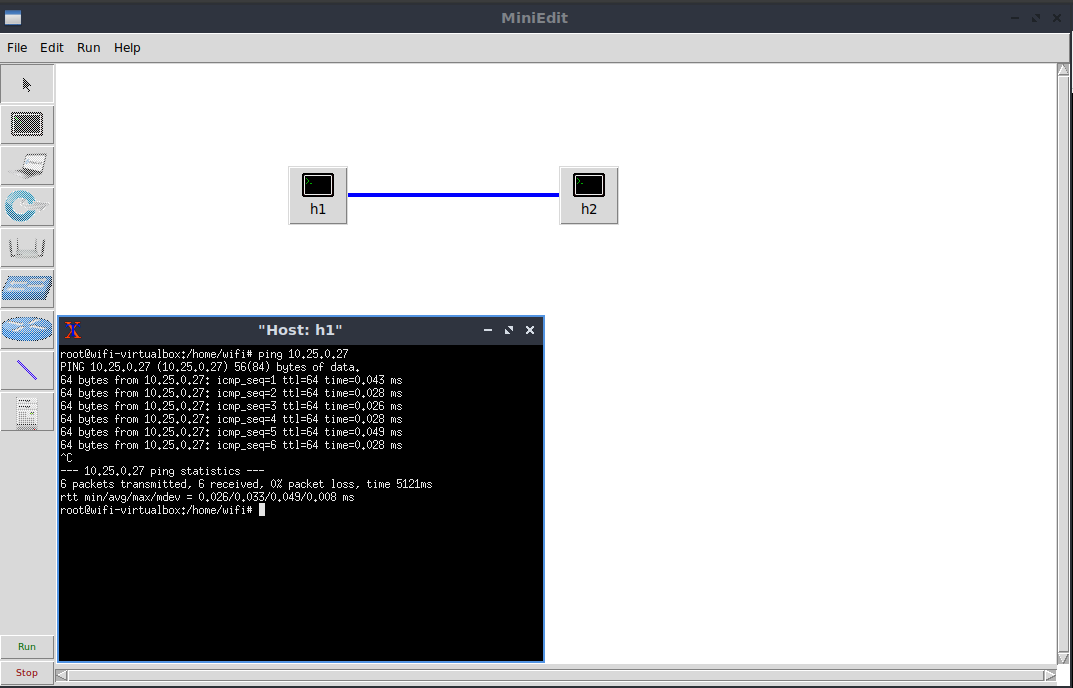
\includegraphics[width=1\textwidth]{./images/T1.1/T1.1TopologyPing.png}
\end{center}
\textbf{1:} `tc qdisc add dev h2-eth0 root netem rate 125mbit`
\begin{center}
    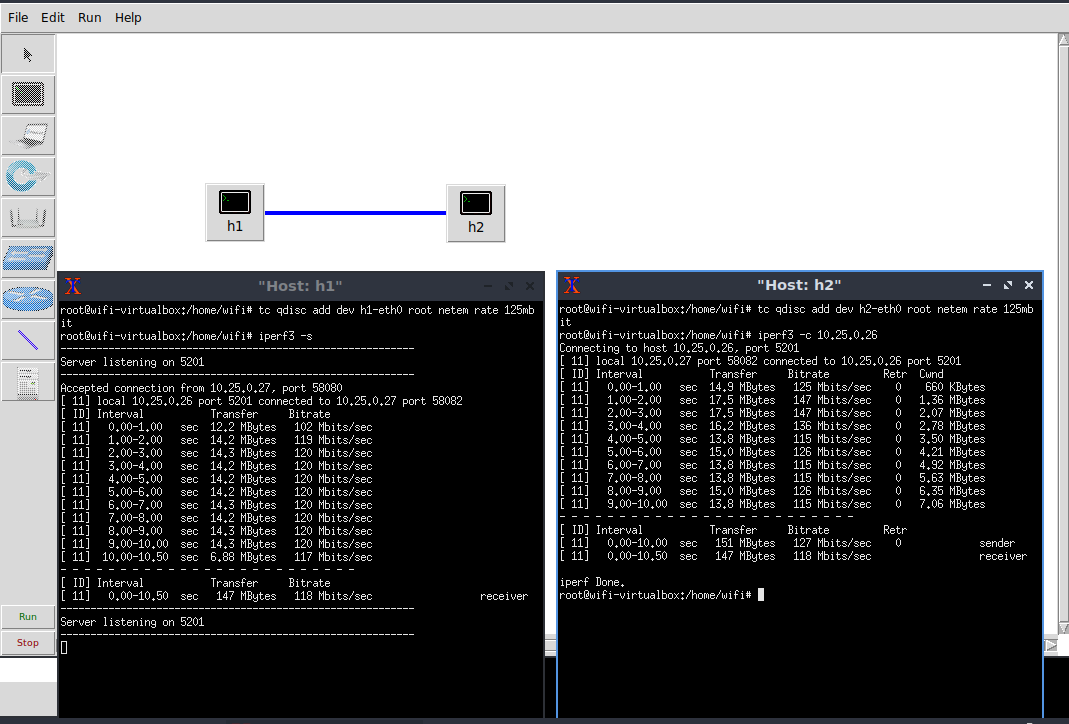
\includegraphics[width=1\textwidth]{./images/T1.1/125test1.png}
    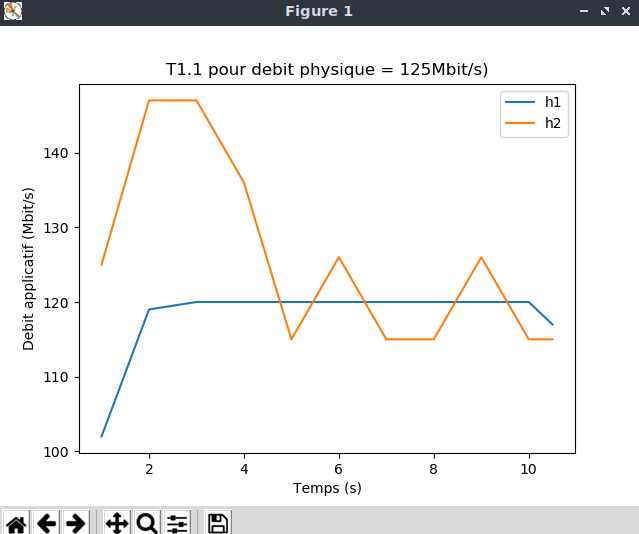
\includegraphics[width=1\textwidth]{./images/T1.1/courbe125test1.png}   
\end{center}
\textbf{Observation :}\\
Débit de H2 (ligne bleue) : Le débit applicatif mesuré sur h1 reste stable autour de 120 Mbps tout au long du test, avec de petites variations entre 102 Mbps et 120 Mbps. Cette stabilité montre que h1 utilise efficacement la limite de 125 Mbps imposée sur le lien, même si ce débit n'est jamais complètement atteint.\\
Débit de H2 (ligne orange) : Le débit applicatif observé sur h2 reste proche de la limite de 125 Mbps, mais présente plus de variabilité par rapport à h1. Le débit oscille avec des pics atteignant 147 Mbps et des baisses à environ 115 Mbps. Ces variations indiquent une certaine instabilité due au réseau.
\vspace{1cm}
\\
\textbf{Explications :} 
\\
La limite de 125 Mbps imposée par tc sur les deux machines fixe un cap clair pour le débit maximal possible, ce qui crée un goulet d’étranglement dans le réseau. Cette limite explique les lectures stables sur h1 autour de 120 Mbps et les performances plus variables sur h2, dues à l’adaptation du protocole TCP. Comme iperf3 utilise TCP, ce dernier ajuste dynamiquement les taux de transfert pour éviter la congestion, adaptant le débit en fonction des retours du réseau. TCP optimise le débit à chaque intervalle et détecte que le lien ne peut dépasser 125 Mbps, donnant ainsi un débit constant pour h1 et plus variable pour h2. Le graphique du débit en fonction du temps montrerait h1 comme une ligne stable proche de 120 Mbps, tandis que h2 oscille autour de 125 Mbps avec des pics et des creux, illustrant la capacité d’adaptation du TCP et le fait que le débit global dépend du maillon le plus lent du réseau.\\
\\
\textbf{2:} `tc qdisc add dev h2-eth0 root netem rate 625mbit `
\begin{center}
    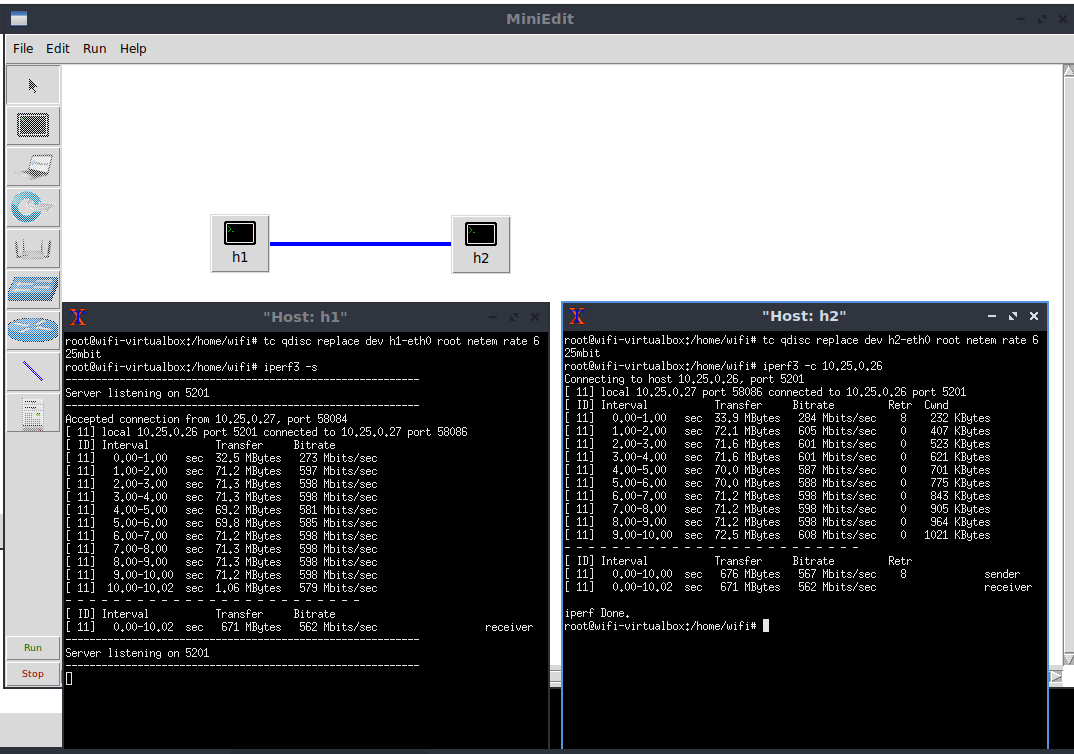
\includegraphics[width=1\textwidth]{./images/T1.1/625test1.png}
    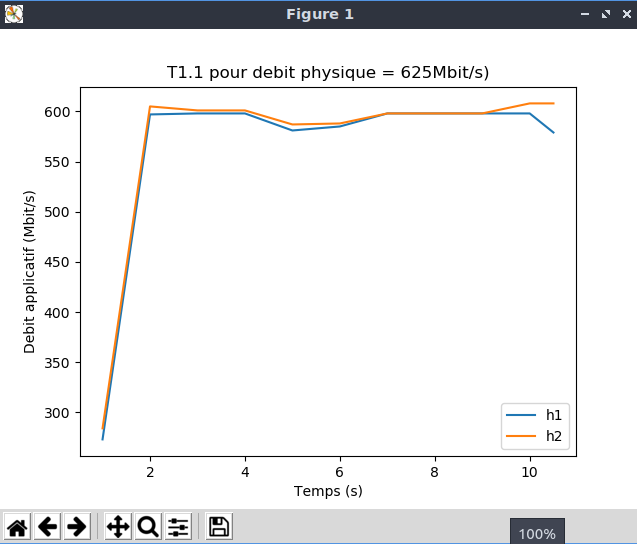
\includegraphics[width=1\textwidth]{./images/T1.1/courbe625test1.png}
\end{center}
\textbf{Observation :}\\
Débit de h1 (ligne bleue) :  Le débit applicatif (débit mesuré) est plus élevé que dans le test précédent, atteignant environ 598 Mbps sur la majorité des intervalles de temps. Bien que le débit commence un peu plus bas à 273 Mbps dans la première seconde, il se stabilise rapidement autour de 598 Mbps, avec quelques fluctuations mineures autour de 581 à 598 Mbps. Cela montre que h1 peut tirer parti de la limite augmentée de 625 Mbps, bien que de légers ajustements se produisent.
Débit de h2 (ligne orange) : Le débit moyen est également proche de la limite fixée de 625 Mbps, avec une stabilité notable entre 587 Mbps et 608 Mbps. Les fluctuations sont faibles, et la congestion window (Cwnd), qui augmente de manière régulière, montre que TCP ajuste son débit de manière progressive pour atteindre un niveau optimal sans congestion. Le débit commence à 284 Mbps dans la première seconde, puis monte rapidement vers le débit maximum proche de 605 Mbps.
\\
\\
\textbf{Explication} :\\
En fixant le débit physique à 625 Mbps avec tc, les deux machines peuvent atteindre un débit supérieur par rapport au test précédent, illustrant l'impact d'un lien plus rapide sur les performances applicatives. Le TCP s’adapte rapidement, et après les premières secondes, il maintient un débit proche de la limite maximale du lien, ce qui est visible dans les valeurs stables des deux machines. Sur h1, la constance autour de 598 Mbps reflète un débit quasi-maximal sans congestion. La légère variabilité observée est due à la réponse de TCP aux capacités du réseau, qui ajuste la transmission pour éviter la surcharge, tout en atteignant presque les 625 Mbps. La congestion window (Cwnd) croissante sur h2 démontre que TCP augmente progressivement le débit en fonction des performances du lien, ce qui permet d’optimiser la transmission sans perte. Le graphique de débit montre une courbe qui monte rapidement pour atteindre le débit stable autour de 600 Mbps, démontrant la capacité du réseau à supporter une charge plus élevée grâce à l’augmentation de la limite de débit.
\vspace{1cm}
\\
\textbf{3:} `tc qdisc add dev h2-eth0 root netem rate 2.5gbit`
\begin{center}
    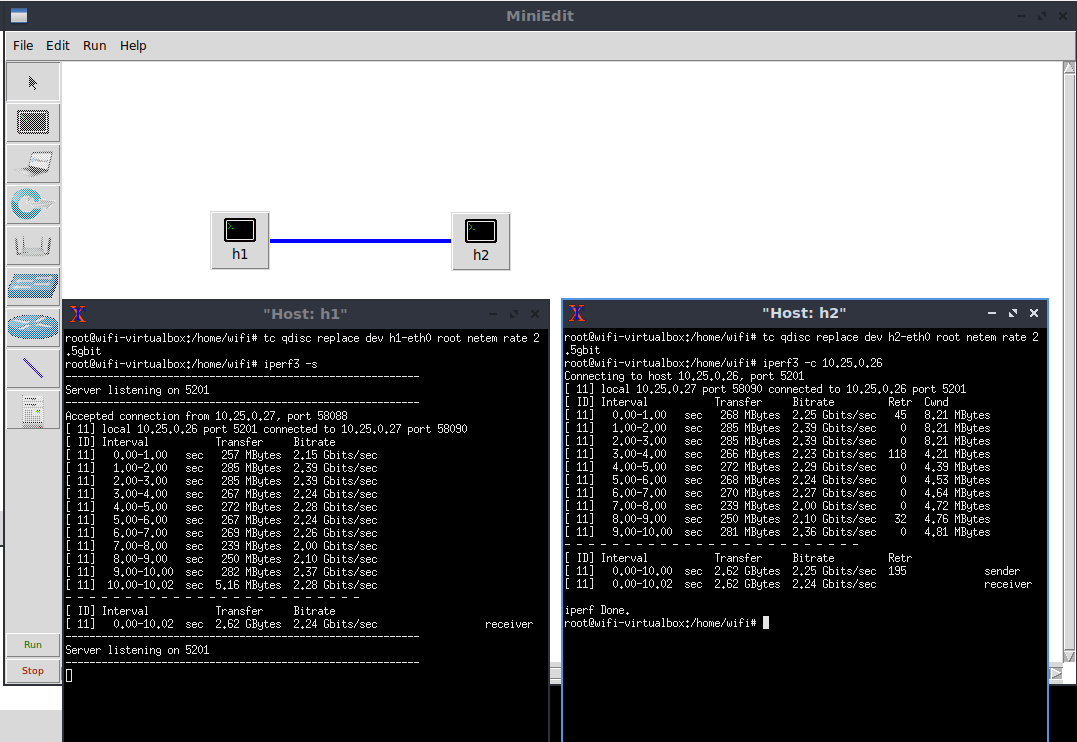
\includegraphics[width=1\textwidth]{./images/T1.1/2500test1.png}
    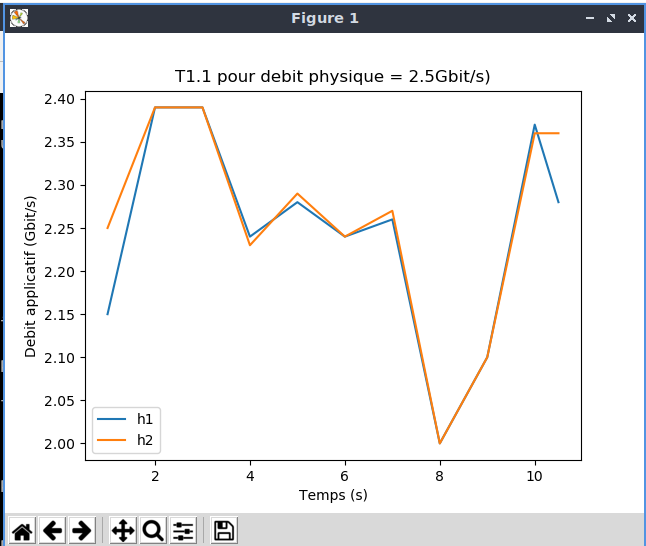
\includegraphics[width=1\textwidth]{./images/T1.1/courbe2500test1.png}
\end{center}
\textbf{Observation :}\\
Débit de h1 (ligne bleue) :  Le débit applicatif est resté stable, autour de 2,37 Gbps en moyenne pendant tout le test. Au début, il y a eu une légère variation, avec un débit un peu plus bas durant la première seconde, mais il s’est rapidement stabilisé entre 2,2 et 2,4 Gbps. Pendant le test, h1 a montré très peu de fluctuations, avec des baisses parfois autour de 2,00 Gbps et des pics à 2,39 Gbps. Cette stabilité montre que h1 utilise efficacement la limite de 2,5 Gbps imposée par tc, en gardant une performance stable et proche du débit maximal autorisé.
Débit de h2 (ligne orange) : De la même manière, h2 a montré une stabilité proche de la limite de 2,5 Gbps, restant en général entre 2,25 et 2,39 Gbps sur la plupart des intervalles. On observe de légères variations, avec des baisses occasionnelles autour de 2,00 Gbps, mais en général g2 suit le même schéma que h1. Le débit moyen est de 2,36 Gbps, ce qui montre que h1 et h2 s’adaptent bien à la vitesse maximale du lien. Bien que h2 présente une légère variabilité, la performance reste globalement stable et alignée avec la limite de 2,5 Gbps.
\\
\\
\textbf{Explication} :\\
Ce test avec une limite de 2,5 Gbps montre une amélioration nette du débit applicatif par rapport aux limites précédentes de 125 Mbps et 625 Mbps. Avec cette nouvelle limite de 2,5 Gbps, TCP s’adapte facilement, ce qui permet au débit applicatif de rester proche du maximum autorisé. Les petites fluctuations initiales, suivies par une stabilisation rapide, illustrent l’ajustement de la fenêtre de congestion (Cwnd) de TCP, qui détecte la vitesse maximale possible avant de se stabiliser.

Contrairement aux cas de 125 Mbps et 625 Mbps, où la limite créait des goulets d’étranglement et exigeait plus d’ajustements de TCP, la vitesse de 2,5 Gbps permet un débit plus élevé sans congestion ni perte de paquets importante. Par conséquent, TCP peut atteindre un débit proche du maximum sans avoir à ajuster fréquemment sa vitesse. Cela montre que le réseau est capable de supporter des charges plus importantes avec peu de latence et de congestion. En général, ces résultats montrent qu’une vitesse de lien plus élevée permet d’augmenter le débit tout en minimisant le besoin d’adaptations de TCP, ce qui rend la transmission plus stable et permet au réseau de gérer des transferts de données plus importants efficacement.
\\
\\
\textbf{4:} `Explication du Graphique Débit Applicatif vs Débit Physique`
\begin{center}
    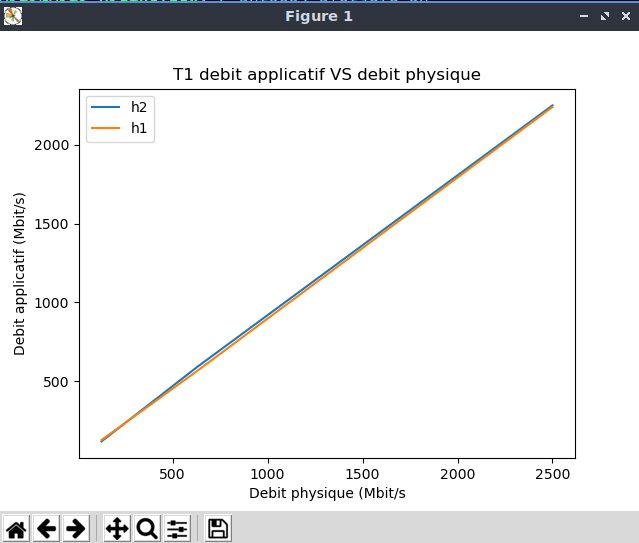
\includegraphics[width=1\textwidth]{./images/T1.1/T1appVSphy.png}
\end{center}
\textbf{Explication} :\\
Le graphique montre une relation linéaire entre le débit physique et le débit applicatif pour les valeurs de 125 Mbps, 625 Mbps et 2,5 Gbps. En augmentant le débit physique, le débit applicatif suit cette progression de façon proportionnelle. Cela signifie que le réseau utilise efficacement la bande passante disponible : plus le débit physique est élevé, plus le débit visible par l’utilisateur est important, sans grande perte ou réduction de performance. Cette linéarité confirme que, dans ces conditions, le réseau n’est pas limité par des goulets d'étranglement majeurs ou de la congestion, et le protocole TCP peut s’adapter pour atteindre le débit maximal permis par la capacité physique du lien.

